\documentclass[12pt]{UoAthesis} 
\usepackage{booktabs} 
\usepackage{color}
\usepackage{graphics}
\usepackage{enumerate}
\thesistitle{Honours Dissertation}
\thesisauthor{Christopher James Thomson} 
\thesispdfkeywords{}
\thesisyear{2012}

\thesisabstract{The objective of this thesis is to determine a general
  technique for converting continuous potentials to equilivant discrete
  potentials. Discrete potentials have many desirable properties. }

\acknowledgements{I would like to dedicate this work to..}

%%% The bibtex file where your references are stored 
\bibliography{main}
\begin{document}

%%% = = = DISSERTATION OVERVIEW = = =

% - INTRODUCTION - %
% Molecules, why are we interested in the molecular scale? What processes are molecular
% - - Molecular dynamics, what is it, why is it important to Chemical
%engineering.

% - - Leading into potentials, need for faster methods, more accurate methods.%
%Review of exisiting literature (Chapela, PRIME SPEADMD), what they've done,
%why its not as good as what you're going to do % 

% Outline of the thesis to come

% - Molecular Simulation 
% -- Newtonian mechanics F=MA, is it valid? 
% -- Forces from potentials (conservative forces) 
% Types of forces (gravitional (which is neglected)), pairwise forces 
% leading to intermolecular potentials.

% --- Give an example soft potential (LJ), Introduce a discrete -- 
% -potential,hard sphere is the prototypical discrete potential, -- 
% -but there are steppedpotentials too (Chapela). Talk about the -- 
% -advantages/disadvantages etc.

%%%% Lead out of the chapter with this 
% --- Introduce discrete potentials, say they need a special method of solution
%(EDMD).
% - Simulation Methods - % 
% - -Force Driven Simulators 
% - - - Introduction and general algorithm 
% - - -Integrators: Euler, Verlet, Velocity Verlet, Gear...lit review to find
%more recent ones
% - - - Optimization: neighbour lists, truncation of the potential 
%- - - Adv/Disadv? or just within other relevant topics 
% - - Event Driven Simulators % - - - Introduction and general algorithm 
% - - - Collision rules 
%Actually older than force based, although not as popular.
% - - - Optimization: neighbour lists, O(1) priority queue algorithms, time warp%algorithms
% - -Measuring System Properties % - - - Radial Distribution Function
 % - - -Temperature 
% - - - Pressure 
% - - - Coefficient of Diffusion 
% - Results - % 
 % - Discussion- % 
% - Conclusions - % 
% - Recommendations for future work - % 
% - Appendices -% 
% - - Derivation of collision rule for stepped potentials %
%% = = = END OVERVIEW = = = %%%

\chapter{Introduction}

Process simulation packages have become an integral part of chemical
engineering design. Central to these simulation software packages is
the ability to calculate thermodynamic and transport properties of
fluids quickly and accurately. Many modern processes rely on molecular
scale effects... (Absorption, membrane technology (reverse osmosis),
catalysis)....

To better understand these large scale systems, we need to improve our
understanding of the smaller scales. Experiments are hard, can't hold
a ruler up to a molecule, everything is too fast, too small to
see. (X-ray crystallography). theory is hard, lots of molecules, can't
solve even three molecules motion analytically (need
cite). simulations are great, don't try to solve analytically. Since
50's (alder wainwright), computers are faster, modern sims are
amazing.

At the heart of these simulations are models for the atoms and
molecules involved. There are two classes of models, discrete and
contiuous.

%paragraph describing the thesis
In chapter~\ref{chap:one}, the something is discussed

\chapter{Molecular Models}
In this chapter, the models used for molecular dynamics (MD)
\nomenclature[A]{MD}{Molecular Dynamics} are discussed. There are two
major types of potentials: continuous and discrete potentials, both
are important to molecular dynamics. The solution to both relies on
the use of classical mechanics to describe the motion of particles.

\section{Classical Mechanics}

\subsection{Validity of Classical Mechanics}

The underlying assumption behind many molecular dynamics simulations
is that the particles move according to the laws of classical
mechanics. Strictly, due to their size and speed, atom and molecules
should be treated using quantum mechanics.  However molecular dynamics
makes a couple of assumptions that allow these quantum mechanical
effects to be ignored.  

The first is the Born-Oppenheimer Approximation which allows the
motion of electrons and the nucleus to be treated separately.  Since
the nucleus is much larger than the electrons and hence less affected
by quantum mechanics, it is treated as a classical particle.  The
electrons on the other hand are represented using a potential \cite{Jasper2006}.

The second assumption is that any quantum mechanical effects should
cancel out. Molecular dynamics is rarely interested in the motion of a
single particle, it is more concerned with the statistical average of
every particle.

These assumtions are usually valid unless very light atoms (such as
hydrogen or helium) are being simulated or the particles are vibrating
at very high rates \cite{Frenkel2002}.

\subsection{Newton's Second Law of Motion \label{NewtonLaw}}

The fundamental identity of newtonian mechnanics is Newton's Second
Law of Motion (equation \eqref{eq:Fma}). This equation allows the prediction of a
particle's trajectory provided that an initial position and velocity
is known; and the forces acting on that particle can be calculated for
any position or velocity.

\begin{equation}
  \mathbf{F} = m\mathbf{a}
  \label{eq:Fma} 
\end{equation}

If a force depends only on the position of a particle it is known as a
conservative force. Almost all forces considered in molecular dynamics
are of this type because atoms or molecules do not lose energy due to
friction or any other dissipative process.

Conservative forces can be of one of two types.  The first are forces
that depend on a particle's absolute position, such as gravity.
However gravity is usually disregarded in MD as atoms and molecules
have such low masses that gravity has very little effect.

The second and most important type are intermolecular forces that
depend on position relative to other particles.  Usually only the
forces between pairs of particles are considered, therefore the total
force acting on a particle $i$ is the sum of the forces between $i$
and every other particle $j$.  This pairwise summation of forces is
shown in equation \eqref{eq:pairwise}, where N is the total number of
particles in the system.

\begin{equation} 
  \mathbf{F}_i = \sum_{j \not= i}^{N}\mathbf{F}_{ij}
  \label{eq:pairwise}
\end{equation}

Force calculations are limited to pairs as this is simpler, but there
are examples of n-body forces such as equation \eqref{eq:tersoff}
\cite{Tersoff1988}.  Here the force between particles $i$ and $j$ is
split into a repulsive force ($\mathbf{F}_R$) and an attractive force
($\mathbf{F}_A$).  The coefficient in front of the repulsive force,
$a$, is a range limiting term, while the coefficient $b$, is the bond
order.  This describes the environment the particles are in, and
strengthens or weakens the attractive force appropriately.

\begin{equation}
  \mathbf{F}_{ij} = a\mathbf{F}_{R} + b\mathbf{F}_A
  \label{eq:tersoff}
\end{equation}

The intermolecular forces used in molecular dynamics are frequently
described using a potential.  Provided that the force is conservative,
it can be calculated from its potential by equation
\eqref{eq:forcePotential}. Here $\nabla$ denotes the gradient of the
potential is the partial differential of the potential in each
orthogonal direction.

\begin{equation} 
  \mathbf{F}=-\nabla \mathcal{U} 
  \label{eq:forcePotential} 
\end{equation}


\section{Continuous Potentials}


A very popular potential used in molecular dynamics simulations is the
Lennard-Jones potential \cite{Lennard-Jones1924} shown in figure
\ref{fig:ljPot} and equation \eqref{eq:LJ} as it is simple yet gives
comparable results to experimental values.

\begin{equation} 
  U(r) = 4 \varepsilon \left[ \left( \frac{\sigma}{r} \right)^{12}
    -\left( \frac{\sigma}{r} \right)^{6} \right] 
  \label{eq:LJ} 
\end{equation}

In equation \eqref{eq:LJ}, $\varepsilon$ is the depth of the energy
well, while $\sigma$ is the distance where the potential between two
particles is zero.

\begin{figure}[htp] 
  \begin{center}
    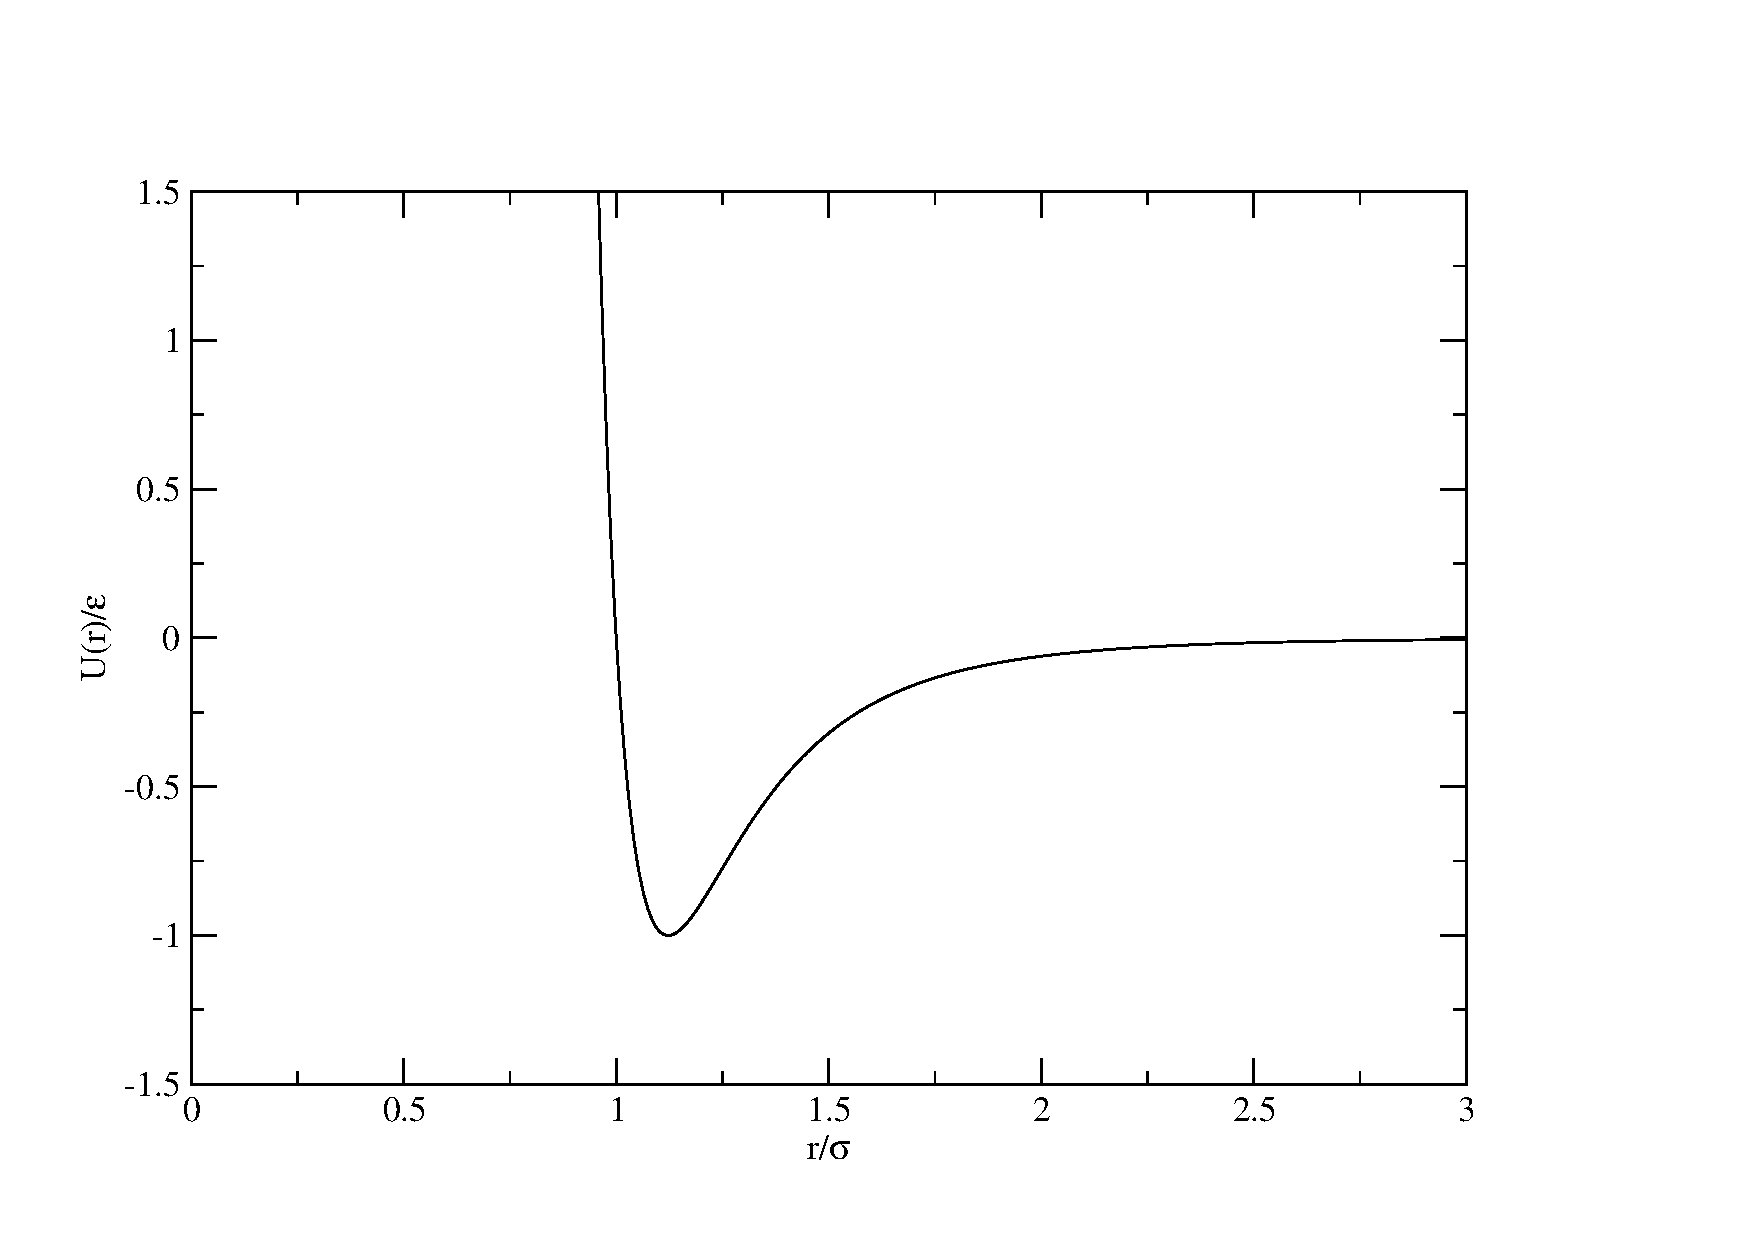
\includegraphics[clip,width=\textwidth]{figures/ljPlot} 
    \caption{\label{fig:ljPot} Plot of the Lennard-Jones potentia} 
  \end{center}
\end{figure}

The power 12 term, $\left(\frac{\sigma}{r}\right)^{12}$ gives the
potential the repulsive core caused by overlapping electron shells,
while the power 6 term, $\left(\frac{\sigma}{r}\right)^{12}$,
represents the attractive Van der Waals forces.  The force between two
Lennard-Jones particles is shown in figure \ref{fig:ljForce}.

\begin{figure}[htp] 
  \begin{center}
    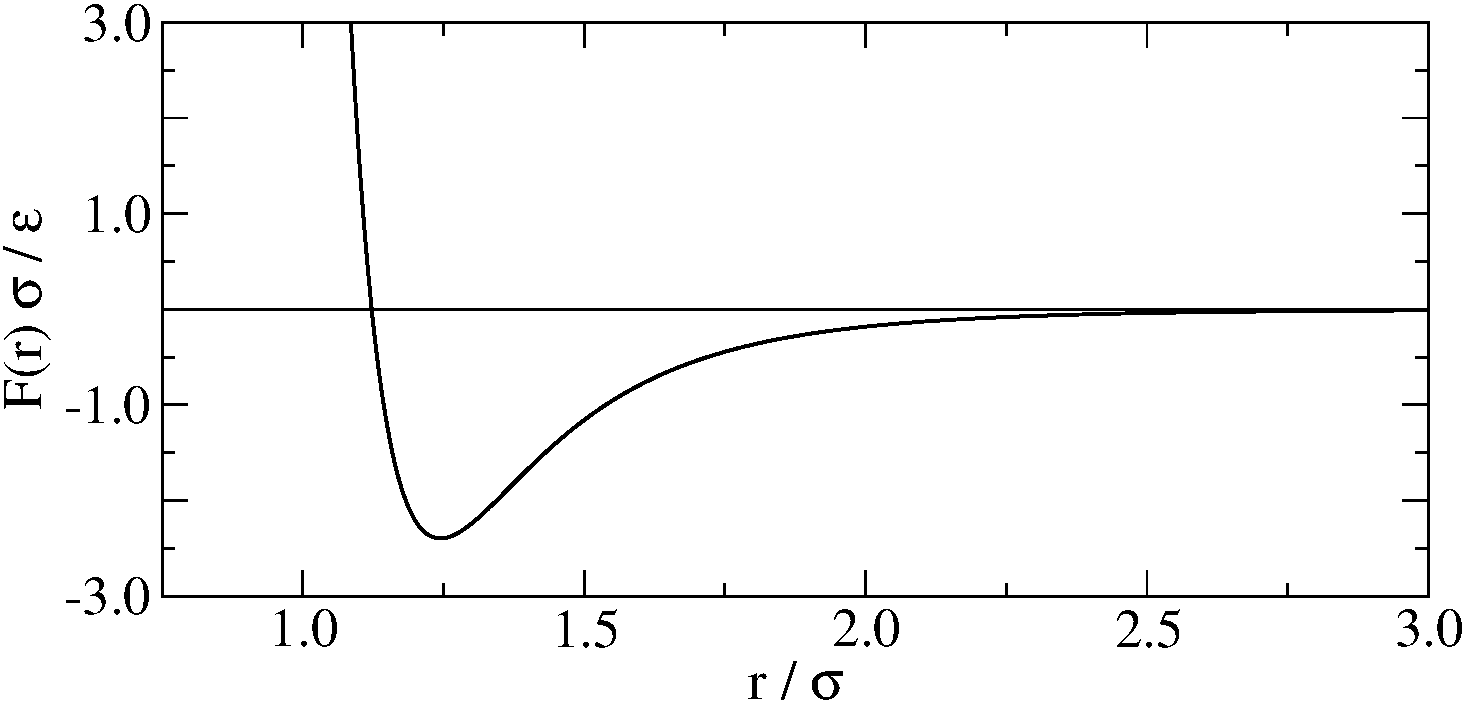
\includegraphics[clip,width=\textwidth]{figures/ljForce} 
    \caption{\label{fig:ljForce} Plot of the force between
      a pair of Lennard-Jones particles separated by a distance $r$}
  \end{center}
\end{figure}

The Lennard-Jones potential is even part of more complex potentials
such as equation \eqref{eq:bigPotential} \cite{Maginn2010}.  Here the
Lennard-Jones potential is used to represent Van der Waals forces while
Coulomb's Law ($\frac{q_iq_j}{r_{ij}}$) is modelling longer range
electrostatic interactions.  The first four terms are contraints on
bond movements (streching, angle bending, ``dihedral angle'' motion,
and out of plane movement of rings respectively).

\begin{align}
  \label{eq:bigPotential}
  \mathcal{U} &= \sum_{\text{bonds}}k_b(r-r_0)^2 
  + \sum_{\text{angles}}k_\theta(\theta - \theta_0)^2 \nonumber\\
  &+ \sum_{\text{dihedrals}} k_\chi[1+\cos(n\chi - \delta)] 
  + \sum_{\text{improper}} k_\psi(\psi - \psi_0)^2 \nonumber\\
  &+ \sum_{i=1}^{N-1}\sum_{j>i}^{N}\left\{ 4 \varepsilon 
    \left[ \left( \frac{\sigma}{r_{ij}} \right)^{12}
      -\left( \frac{\sigma}{r_{ij}} \right)^{6} \right] 
    + \frac{q_iq_j}{r_{ij}}\right\}
\end{align}

\section{Discrete Potentials}

Discrete potentials differ from continuous potentials because they
have discontinuities.  The simplest discrete potential is that of the
hard sphere.

Hard spheres were the first type of particles simulated
\cite{Alder1957} due to their relative simplicity.  The potential for
hard spheres is shown in equation \eqref{eq:potentialHS}, where $\sigma$
is the diameter of the spheres.

\begin{equation}
  \label{eq:potentialHS}
  \mathcal{U} = 
  \begin{cases}
    \infty &\text{if }\; |\mathbf{r}_i - \mathbf{r}_j| < \sigma \\
    0 &\text{if }\; |\mathbf{r}_i - \mathbf{r}_j| > \sigma
  \end{cases}
\end{equation}

The hard sphere potential can be elaborated upon by adding an
attractive well out side the hard core.  This square well potential
takes the form of equation \eqref{eq:potentialSW} \cite{Barker1967},
where $\lambda$ is the outer radius of the core in terms of the hard
core diameter $\sigma$.

\begin{equation}
  \label{eq:potentialSW}
  \mathcal{U} = 
  \begin{cases}
    \infty &\text{if }\; |\mathbf{r}_i - \mathbf{r}_j| < \sigma \\
    -\varepsilon &\text{if }\; \sigma < |\mathbf{r}_i - \mathbf{r}_j| < \lambda\sigma \\
    0 &\text{if }\; |\mathbf{r}_i - \mathbf{r}_j| > \lambda\sigma
  \end{cases}
\end{equation}

The square well potential is similar to the Lennard-Jones potential in
that they have an attractive well, followed by a steep repulsive core,
however the two give quite different simulation results.  


Hence people have created better discrete potentials to model molecular interactions
 Hard sphere,

square well -> compare to LJ

SPEAMD, PRIME

Lead out with the two methods used to simulate these potentials are quite different....




\chapter{Molecular Dynamics}

\section{Force-driven Simulators} 
In order to compare the effectiveness of step potentials a set of
comparison results from a continuous potential is needed.  The method
to simulate a continuous potential is given in this section.

Force-driven (or time driven) simulators are the most popular method
of simulating particles due to their relative simplicity and ability
to handle continuous potentials. Simulators of this kind were
pioneered by Rahman \cite{Rahman1964} who predicted physical
properties of liquid argon using a Lennard-Jones potential with
reasonable accuracy.

The distinguishing feature between force-driven and event-driven
simulators is the way in which they move through time. During
force-based simulations particles' positions and velocities are
calculated at uniform intervals of time, $\Delta t$ using the forces
acting on the particles. These newly calculated values are then used
to predict the next set of particle positions. This is then repeated
over the desired simulation time.

The general algorithm for a force driven simulator is as follows. 
\begin{flushleft}
  \begin{enumerate} 
  \item Initialisation 
  \item Calculate particles' future positions 
  \item Calculate the forces acting on the particles 
  \item Calculate the future velocities of particles 
  \item Run thermostat (if enabled) 
  \item Measure properties 
  \item Repeat steps 2-6 for the desired number of iterations
  \end{enumerate} 
\end{flushleft}

\subsection{Initialisation \label{sec:initMD}} The particles are initialised in a Face Centered
Cubic (FCC) \nomenclature[A]{FCC}{Face Centered Cubic} structure. The
use of the FCC lattice is common when simulating Lennard-Jones
potentials as the first force-driven simulation \cite{Rahman1964} was
carried out using liquid Argon which crystalises to a FCC lattice.

Particle velocities are assigned randomly from a Gaussian distribution
with a mean, $\mu = 0$, and a standard deviation, $\sigma =
\sqrt{T^{*}}$, where $T^{*}$ is the desired reduced temperature. The
velocities are then rescaled to ensure there net shift in linear
momentum in any direction by applying \eqref{eq:zeroLinearP} in each
orthongonal direction.

\begin{equation} 
  v_{i}^{new} = v_{i}^{old} - \frac{1}{N}
  \sum^{N}_{i}v_{i}^{old}
  \label{eq:zeroLinearP} 
\end{equation}

\subsection{Integrators} 

Predicting the particles' future positions require solving Newton's
Second Law of Motion (equation \ref{eq:Fmvdot}), using forces
calculated from the potential.

\begin{equation} 
  \mathbf{F} = m \frac{\partial^2 \mathbf{r}}{\partial t^2}
  \label{eq:Fmvdot} 
\end{equation}

However, since acceleration is the second time derivative of position
(velocity is the first time deriviative), calculating the particle's
future position results in solving a differential equation. In order
to accomplish this numerical integrators are used.

The majority of numerical integrators are based on Taylor Series
(equation \ref{eq:Taylor}).

\begin{equation} 
\mathbf{r}(t+\Delta t) = \mathbf{r}(t) + 
\frac{\partial\mathbf{r}(t)}{\partial t}(\Delta t) + 
\frac{1}{2}\frac{\partial^2\mathbf{r}(t)}{\partial t^2}\Delta t^2 + 
\frac{1}{3!}\frac{\partial^3\mathbf{r}(t)}{\partial t^3}\Delta t^3 
+ \frac{1}{4!}\frac{\partial^4\mathbf{r}(t)}{\partial t^4}\Delta t^4 
+ ... \label{eq:Taylor} 
\end{equation}

The simplest integrator is Euler's Method which is just the Taylor
Series truncated after the acceleration term (equation
\ref{eq:Euler}).

\begin{equation} 
  \mathbf{r}(t+\Delta t) = \mathbf{r}(t) + \mathbf{v}(\Delta t) +
  \frac{1}{2}\mathbf{a}\Delta t^2 + \mathcal{O}(\Delta t^3) 
  \label{eq:Euler}
\end{equation}

However this method suffers from large errors and is highly unstable
(i.e.\ it amplifies any errors) \cite{Haile1997} and is therefore rarely
used. The Verlet Integrator \cite{Verlet1967} improves upon Euler's
method by combining the forward timestep with a reverse timestep
\eqref{eq:Verletpos}. This method is actually fourth order as the
third (and first) derivative is cancelled out during its
derivation. The Verlet integrator does not include an equation to
calculate the future velocity so the central difference used by Verlet
is often used \eqref{eq:VerletVel}.

\begin{subequations} 
  \begin{align} 
    \mathbf{r}(t + \Delta t) &= 2\mathbf{r}(t) - \mathbf{r}(t - \Delta t) 
    + \mathbf{a}(t)\Delta t^2 + \mathcal{O}(\Delta t^4)
    \label{eq:Verletpos} \\
    \mathbf{v}(t+\Delta t) &= \frac{\mathbf{r}(t+\Delta t) -
      \mathbf{r}(t-\Delta t)}{2\Delta t} 
    \label{eq:VerletVel} 
  \end{align}
\end{subequations}

Integrators suffer from couple key failings that cause a systematic
gain of energy known as ``energy drift''. Firstly, integrators are
based on infinite Taylor series which cannot be fully implemented,
therefore they have to be truncated after a certain number of terms,
this introduces an error. Secondly, integrators struggle to predict
values of forces that have discontinuities in them, such as discrete
potentials or discontinuities introduced by truncating potentials to
improve simulator speed.  There are a couple of types of integrators
that try and reduce these problems.

The first method to improve the traditional integrator is the
predictor-corrector integrator. These use a truncated Taylor series
to calculated a predicted value for the future position and higher
order time derivatives. The force is then calculated at this
predicited position, then the difference between the predicted
acceleration and the corrected acceleration calculated from the force
is used to correct the position and time derivatives.

The most popular predictor-corrector integrator is that of Gear
\cite{Gear1971},using his 5th order algorithm. The predicted value for
the $i^{th}$ time derivative is shown in \eqref{eq:GearPredictor}, and
defining $\Delta \mathbf{a} = \mathbf{a}\,^{C} - \mathbf{a}\,^{P}$, the
corrected time derivatives can be calculated using
\eqref{eq:GearCorrector} with coefficients from \eqref{eq:GearCoeff}.

\begin{equation} 
  \frac{\partial^{i}}{\partial t^{i}} \mathbf{r}\:^{P}(t+\Delta t)
  =\sum^{n}_{k=i} \frac{1}{k!}\frac{\partial^{i} }{\partial t^{i}}
  \mathbf{r}(t) \Delta t^{k} 
  \label{eq:GearPredictor} 
\end{equation}

\begin{equation} 
  \frac{\partial^{i}}{\partial t^{i}} \mathbf{r}\:^{C}(t+\Delta t)
  =\frac{\partial^{i} }{\partial t^{i}} \mathbf{r}\:^{P}(t+\Delta t)
  +\frac{c_i}{\Delta t^i} \left(\frac{\Delta t^2}{2}\Delta \mathbf{a}\right)
  \label{eq:GearCorrector} \end{equation} \begin{equation} c_0 =
  \frac{3}{16},\;\;c_1 = \frac{251}{360},\;\; c_2 = 1,\;\; c_3 =
  \frac{11}{18},\;\; c_4 =
  \frac{1}{6},\;\; c_5 = \frac{1}{60} \label{eq:GearCoeff} 
\end{equation}

The Gear's algorithm, while more accurate at short timesteps than Verlet's
integrator \cite{Haile1997}, suffers at long timesteps and is computationally
more expensive.

The other method used to try and mitigate the failings of other types
of integrator is the sympletic integrator.  These have the useful
property in that they, on average, conserve energy
\cite{Hairer2003}. The most common symplectic integrator used in MD is
the Velocity Verlet Integrator \cite{Swope1982} shown in
\eqref{eq:VVerlet}.

\begin{subequations}
\label{eq:VVerlet}
\begin{align}
 \mathbf{r}(t + \Delta t) &= \mathbf{r}(t) + \mathbf{v}(t) \Delta t 
 + \frac{1}{2}\mathbf{a}(t) \Delta t^2 + \mathcal{O}(\Delta t^4)
 \label{eq:VVerletpos} \\
 \mathbf{v}(t+\Delta t) &= \mathbf{v}(t) + \frac{\mathbf{a}(t) 
   + \mathbf{a}(t+\Delta t)}{2}\Delta t
 \label{eq:VVerletVel}
\end{align}
\end{subequations}

The popularity of the Velocity Verlet is due to its computational
simplicity and its accuracy and stability at relatively long
timesteps. It can even be expanded\cite{Khakimov2002} to maintain its
accuracy and stability at very long timesteps at a small extra
computational cost. However the Velocity Verlet cannot be used in
systems that do not conserve energy, ie systems with dissipative
forces.

Since in this disseration all forces considered are conservative the
Velocity Verlet integrator is used.

\subsection{Periodic Boundary Conditions}

When simulating a system it is necessary to have a boundary to prevent
the particles from moving away from each into infinity.  However solid
walls have a large effect on the properties of a system so an
alternative method is needed.  Since some of the earliest MD
simulations \cite{Alder1959} have used periodic boundary conditions to
solve this problem.  

\begin{figure}[htp] 
  \begin{center}
    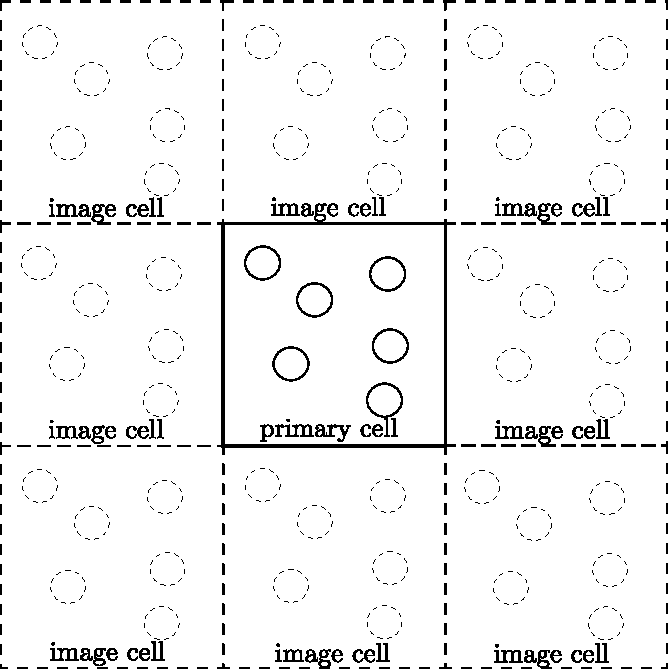
\includegraphics[clip, scale = 0.8]{figures/PBC} 
    \caption{\label{fig:PBC} Figure showing 2D periodic boundary
      conditions. Only the nearest 8 images (dashed) to the simulated
      system (solid) are shown.}
  \end{center}
\end{figure}

The concept behind periodic boundary conditions is to create a
pseudoinfinite system made up of tessellated images of the simulated
system (as shown in figure \ref{fig:PBC}).  When a particle leaves the
primary cell, its image enters from the opposite side.  This ensures
mass is conserved in each cell.  This, however, brings the problem of
particles being able to interact with multiple images of another
particle, or even with themselves.  The minimum image criterion is
used to ensure particles only interact with the closest image of
another particle.


\subsection{Thermostat}

All simulations in this dissertation used the caniocal NVT ensemble,
i.e.\ the number of particles, $N$; the volume of the system, $V$ and
the temperature, $T$ were kept constant during the simulation.  While
keeping the number of particles and system size constant is simple,
controlling the temperature is more complex.  

The simplest method for controlling the temperature is to rescale the
particle velocities to match the desired temperature using equation
\eqref{eq:tempRescale}. 

\begin{equation}
  \label{eq:tempRescale}
  \mathbf{v}_{\text{new}} = \mathbf{v}_{\text{old}} \sqrt{\frac{T_{\text{desired}}}{T_{\text{current}}}}
\end{equation}

However this does not allow energy fluctuations that should exist in a
NVT system, therefore an Andersen thermostat\cite{Andersen1980} is
used.  An Andersen thermostat works by colliding a random particle
with a ghost particle at the desired temperature.  In this
force-driven simulation, this is achieved by reassigning the
velocities of 5\% of particles from a Gaussian distribution at the
correct temperature (similar to section \ref{sec:initMD}).

\subsection{Optimisation}

Due to the time-consuming nature of computer simulations there are a
number of techniques used to speed up simulations.  Since the
calculation of the forces on the particles is the most time-consuming
part of force-driven simulations \cite{Frenkel2002}, almost all
optimising techniques focus on this aspect.

The first technique to improve simulation speed is to truncate the
potential.  Since continuous potentials tend to zero as particles get
further away from each other, significant time can be saved by
selecting a cut-off radius at which the potential is taken to be zero.
The form of a truncated potential is shown in equation
\eqref{eq:truncatePotential}.  For the Lennard-Jones potential a
cut-off radius of $3\sigma$ is used as $\mathcal{U}(3\sigma) =
-0.00548\varepsilon$ and $F(3\sigma) = -0.0109\varepsilon/\sigma$ are
both approximately 1\% of the minimum values.

\begin{equation}
  \label{eq:truncatePotential}
  \mathcal{U}(r) = 
  \begin{cases}
    \mathcal{U}(r) &\text{if }\; r \leq r_{\text{cut-off}} \\
    0 & \text{if }\; r > r_{\text{cut-off}} 
  \end{cases}
\end{equation}

While truncating the potential prevents the calculation of the forces
it still requires the computation of the distance between particles.
These extraneous calculations can be eliminated by using a neighbour list.

There are two main types of neighbour list used in molcular dynamics
simulations.  The first is the use of Verlet lists \cite{Verlet1967},
and this is the type used in this disseration for the force-driven
simulation.  A Verlet list is a list of all the particles within a
certain radius of a particle.  If this list was updated every
timestep, this would be no improvement on the original method, but by
making the Verlet radius larger than the truncation radius, these list
can be used for multiple timesteps.  Haile \cite{Haile1997} recommends
using a Verlet radius of $3.3\sigma$, and updating the list every $10$
timesteps, and this is what was done in this dissertation.

Another method is to use cell-linked lists \cite{Poschel2005}, this
method involves dividing the system into a grid and only the particles
in the same cell or a neighbouring cell are taken into account.  This
method can however be inefficient as the length of each cell must be
at least the truncation cut-off radius wide to prevent particles being
missed out.  However this means a volume of $27r_{\text{cut-off}}^3$
(as in 3 dimensions each cell has 26 neighbours) are considered but
only particles within the spherical volume $\frac{4}{3}\pi
r_{\text{cut-off}}^3$ should be checked; this means the volume checked
is over six times larger than it needs to be.  

Mattson and Rice \cite{Mattson1999} improve this by reducing the
length of each cell to less than the cut-off radius, but this results
in more neighbouring cells having to be checked i.e. for a cell length
of $0.5r_{\text{cut-off}}$ the nearest 124 (a $5\times 5\times 5$
grid) cells are considered neighbours. This means there is a
compromise as smaller cells mean that less volume is checked, but also
means the cell lists are made obsolete quicker and therefore have to
generated more frequently.

 \newpage
\section{Event-Driven Simulators}
 
Start off by pointing out that discontinuous potentials have
discontinuities! Whats the force on these points? Infinity! Can't
integrate over these discontinuities, but what about between them? We
can solve F=ma, (solve it). We can then analytically integrate
newton's equation of motion. We can then try to detect when a
discontinuity occurs and treat them as they happen.

How do you solve what happens over a discontinuity? Conservation of
momentum and energy (see appendix).

\subsection{Introduction} 

Most molecular dynamics simulations use potentials to calculate the
forces acting on particles (see section \ref{NewtonLaw}), however this
is problematic when using discrete potentials.  The gradient (and
hence the force) is either infinite at the steps or zero between them.

Therefore a new technique for simulating these discrete potentials is
needed.  Since between the steps there is no force therefore the
acceleration (and higher order time derivatives) are zero the Taylor
series (equation \eqref{eq:Taylor}) can be reduced to equation
\eqref{eq:edNewPos}.

\begin{equation}
  \mathbf{r}(t+\Delta t) = \mathbf{r}(t) + \mathbf{v}(t)\Delta t 
  \label{eq:edNewPos}
\end{equation}

This leaves only the problem of simulating the point where the
particles are at a step, but since, energy and momentum must be
conserved, this too can be overcome (this is expanded upon in section
\ref{sec:CollDyn}).  This method is known as event-driven molecular
dynamics.

Though force-driven simulators are more popular the first MD
simulation was done using an event-driven simulator by Alder and
Wainwright \cite{Alder1957}. Event-driven simulators differ from
force-driven simulators in that they move through time by jumping from
the point when a discontinuity occurs (known as a collision) to the
next discontinuity.  These collisions are taken to be instantaneous
and only one can occur at any particular time.

The general algorithm for a event driven simulator shown below.

\begin{flushleft}
  \begin{enumerate} 
  \item Initialisation 
    \begin{enumerate}[i.]
      \item Initialise particles
      \item Initialise event list
      \item Initialise capture map
    \end{enumerate}
  \item Find the next event
  \item Process the event
  \item Update the event list
  \item Measure properties 
  \item Repeat steps 2-5 for the desired number of events
  \end{enumerate} 
\end{flushleft}

This algorithm is more complex than that for the force driven
simulation especially when event-driven simulators generally have many
different types of event.


\subsection{Collision Time Prediction}
The initialisation of the particles for the event-driven simulation is
identicle to that for the force-driven simulation.densityNIST An event-driven
simulator first must calculate the collision times between every pair
of particles (provided the particles do collide), in order to select
the earliest collision.  For hard sphere simulations there are two
conditions that must be satisfied in order for a collision to occur.
Firstly, the particles must be moving towards each other and secondly,
the particles must pass close enough to each other to collide.  These
conditions can be expressed mathematically in equations
\eqref{eq:collConditions1} and \eqref{eq:collConditions2} respectively
\cite{Haile1997}.

\begin{subequations}
  \begin{align}
    \mathbf{v}_{ij}\cdot\mathbf{r}_{ij} < 0 \label{eq:collConditions1}\\
    (\mathbf{v}_{ij}\cdot\mathbf{r}_{ij})^2 
    - v_{ij}^2(r_{ij}^2 - \sigma^2) \geq 0 \label{eq:collConditions2}
  \end{align}
\end{subequations}

The time to collision can then be calculated using the quadratic in
equation \eqref{eq:collEnterTime}.  While there are two solutions,
only the earliest collision (the negative root) needs to be
considered.  The second root gives the time when the particles leave
after passing through each other which, for hard sphere, cannot
happen.

\begin{equation}
\Delta t = \frac{(-\mathbf{v}_{ij}\cdot\mathbf{r}_{ij}) \pm 
  \sqrt{(\mathbf{v}_{ij}\cdot\mathbf{r}_{ij})^2 - v_{ij}^2(r_{ij}^2 - \sigma^2)}}
       {v_{ij}^2} \label{eq:collEnterTime}
\end{equation}

Since $\mathbf{v}_{ij}\cdot\mathbf{r}_{ij}$ must be negative for the
collision, there is the possibility of catastrophic cancellation
\cite{Goldberg1991}, if $(\mathbf{v}_{ij}\cdot\mathbf{r}_{ij})^2 \gg
v_{ij}^2(r_{ij}^2 - \sigma^2)$. Therefore it is advisable to use the
positive root from the alternate form of the quadratic equation given
in equation \eqref{eq:collEnterTimeAlt} \cite{Poschel2005}.

\begin{equation}
\Delta t = \frac{r_{ij}^2 - \sigma^2}{(-\mathbf{v}_{ij}\cdot\mathbf{r}_{ij})
  \mp \sqrt{(\mathbf{v}_{ij}\cdot\mathbf{r}_{ij})^2 
    - v_{ij}^2(r_{ij}^2 - \sigma^2)}}
\label{eq:collEnterTimeAlt}
\end{equation}

When considering stepped potentials many of the same principles apply,
except there are now two possible ``collisions''. The first, when two
particles enter a step is treated identically to hard spheres. The
other event, when the particles leave the step, is calculated using
the second, later root of the quadratic.  In order to prevent loss of
numerical precision, the leaving time should be calculated using
equation \eqref{eq:collExitTime}.

\begin{equation}
  \label{eq:collExitTime}
\Delta t = 
\begin{cases}
  \frac{r_{ij}^2 - \sigma^2}{(-\mathbf{v}_{ij}\cdot\mathbf{r}_{ij})
    - \sqrt{(\mathbf{v}_{ij}\cdot\mathbf{r}_{ij})^2 
      - v_{ij}^2(r_{ij}^2 - \sigma^2)}}, & \text{if }
  \mathbf{v}_{ij}\cdot\mathbf{r}_{ij} > 0 \\
\\

\frac{(-\mathbf{v}_{ij}\cdot\mathbf{r}_{ij}) +
  \sqrt{(\mathbf{v}_{ij}\cdot\mathbf{r}_{ij})^2 - v_{ij}^2(r_{ij}^2 - \sigma^2)}}
     {v_{ij}^2} , & \text{if }
     \mathbf{v}_{ij}\cdot\mathbf{r}_{ij} < 0 
\end{cases}
\end{equation}

\subsection{Collision Dynamics \label{sec:CollDyn}}
Once the time of the next collision is known, the particles can be moved
to their new locations.  Generally there is no external force applied
to the particles in event-driven molecular dynamics, therefore the
particles move in straight lines.  Hence the particles' new positions
can be calculated using equation \eqref{eq:edNewPos}.



The post-collision velocities of the colliding particles must now be
calculated.  The simplest collision between two particles is an
elastic bounce, where the velocities and just exchanged along the
separation vector between the two particles.  The change in velocity
during the collision for particles $i$ and $j$ is shown in equation
\eqref{eq:postVBounce}.

\begin{subequations}
  \label{eq:postVBounce}
  \begin{align}
    \Delta\mathbf{v}_i &= -(\mathbf{v}_{ij}\cdot\mathbf{\hat{r}}_{ij})\mathbf{\hat{r}}_{ij} \\
    \Delta\mathbf{v}_j &= (\mathbf{v}_{ij}\cdot\mathbf{\hat{r}}_{ij})\mathbf{\hat{r}}_{ij}
  \end{align}
\end{subequations}

For stepped potential system, the collision dynamics are more complex.
When two particles collide they must pay an energy ``cost'' to proceed
through the step.  This energy cost $\Delta U$ is the difference in
the energy of the current step and the step the particles are going
into, and is shown in equation \eqref{eq:energyCost}.

\begin{equation}
  \label{eq:energyCost}
  \Delta U = U_{\text{next step}} - U_{\text{current step}}
\end{equation}

If the kinect energy of the particles is insufficient, the pair bounce
off the step and the post-collision velocities are calculated using
equation \eqref{eq:postVBounce}. However, if the particles can pay
this cost i.e.\ the inequality \eqref{eq:kineticCost} is true, then the
particles can enter the step.

\begin{equation}
\label{eq:kineticCost}
  \frac{1}{4}m(\mathbf{v}_{ij}\cdot\mathbf{\hat{r}}_{ij})^2 > \Delta U
\end{equation}

The change in the velocities of particles $i$ and $j$ after going
through a step are shown in equation \eqref{eq:postVCapture} where $A$
is given in equation \eqref{eq:changeMomentum}, the derivation of
these equations is given in Appendix ???.  If the particles are
entering a step, the positive root of $A$ is used, whereas if the
particles are leaving a step it is the negative root that should be
used.

\begin{subequations}
  \label{eq:postVCapture}
  \begin{align}
    \Delta\mathbf{v}_i &= \frac{A}{m} \mathbf{\hat{r}}_{ij} \\
    \Delta\mathbf{v}_j &= -\frac{A}{m}\mathbf{\hat{r}}_{ij}
  \end{align}
\end{subequations}

\begin{equation}
  \label{eq:changeMomentum}
  A = -\frac{m}{2}\left((\mathbf{v}_{ij}\cdot\mathbf{\hat{r}}_{ij}) \pm
  \sqrt{(\mathbf{v}_{ij}\cdot\mathbf{\hat{r}}_{ij})^2 - \frac{4}{m}\Delta U}\right)
\end{equation}
\newpage

\newpage

\chapter{Measuring Thermodynamic Properties}
\section{Introduction}
Molecular dynamics is a useful tool to predict macroscopic properties
of particles systems.  Many of the identities and methods to measure
these properties are derived in statistical mechanics.  However, even
when the system is at equilibrium, these properties fluctuate around a
mean (see figure \ref{fig:fluctuations}) therefore it is common to
take time averages of these values. These time averages are denoted
with angle brackets $\langle\:\: \rangle$, and the time average of a
property, $A$, is shown in \eqref{eq:TAdef} \cite{Haile1997}.

\begin{figure}[htp] 
  \begin{center}
    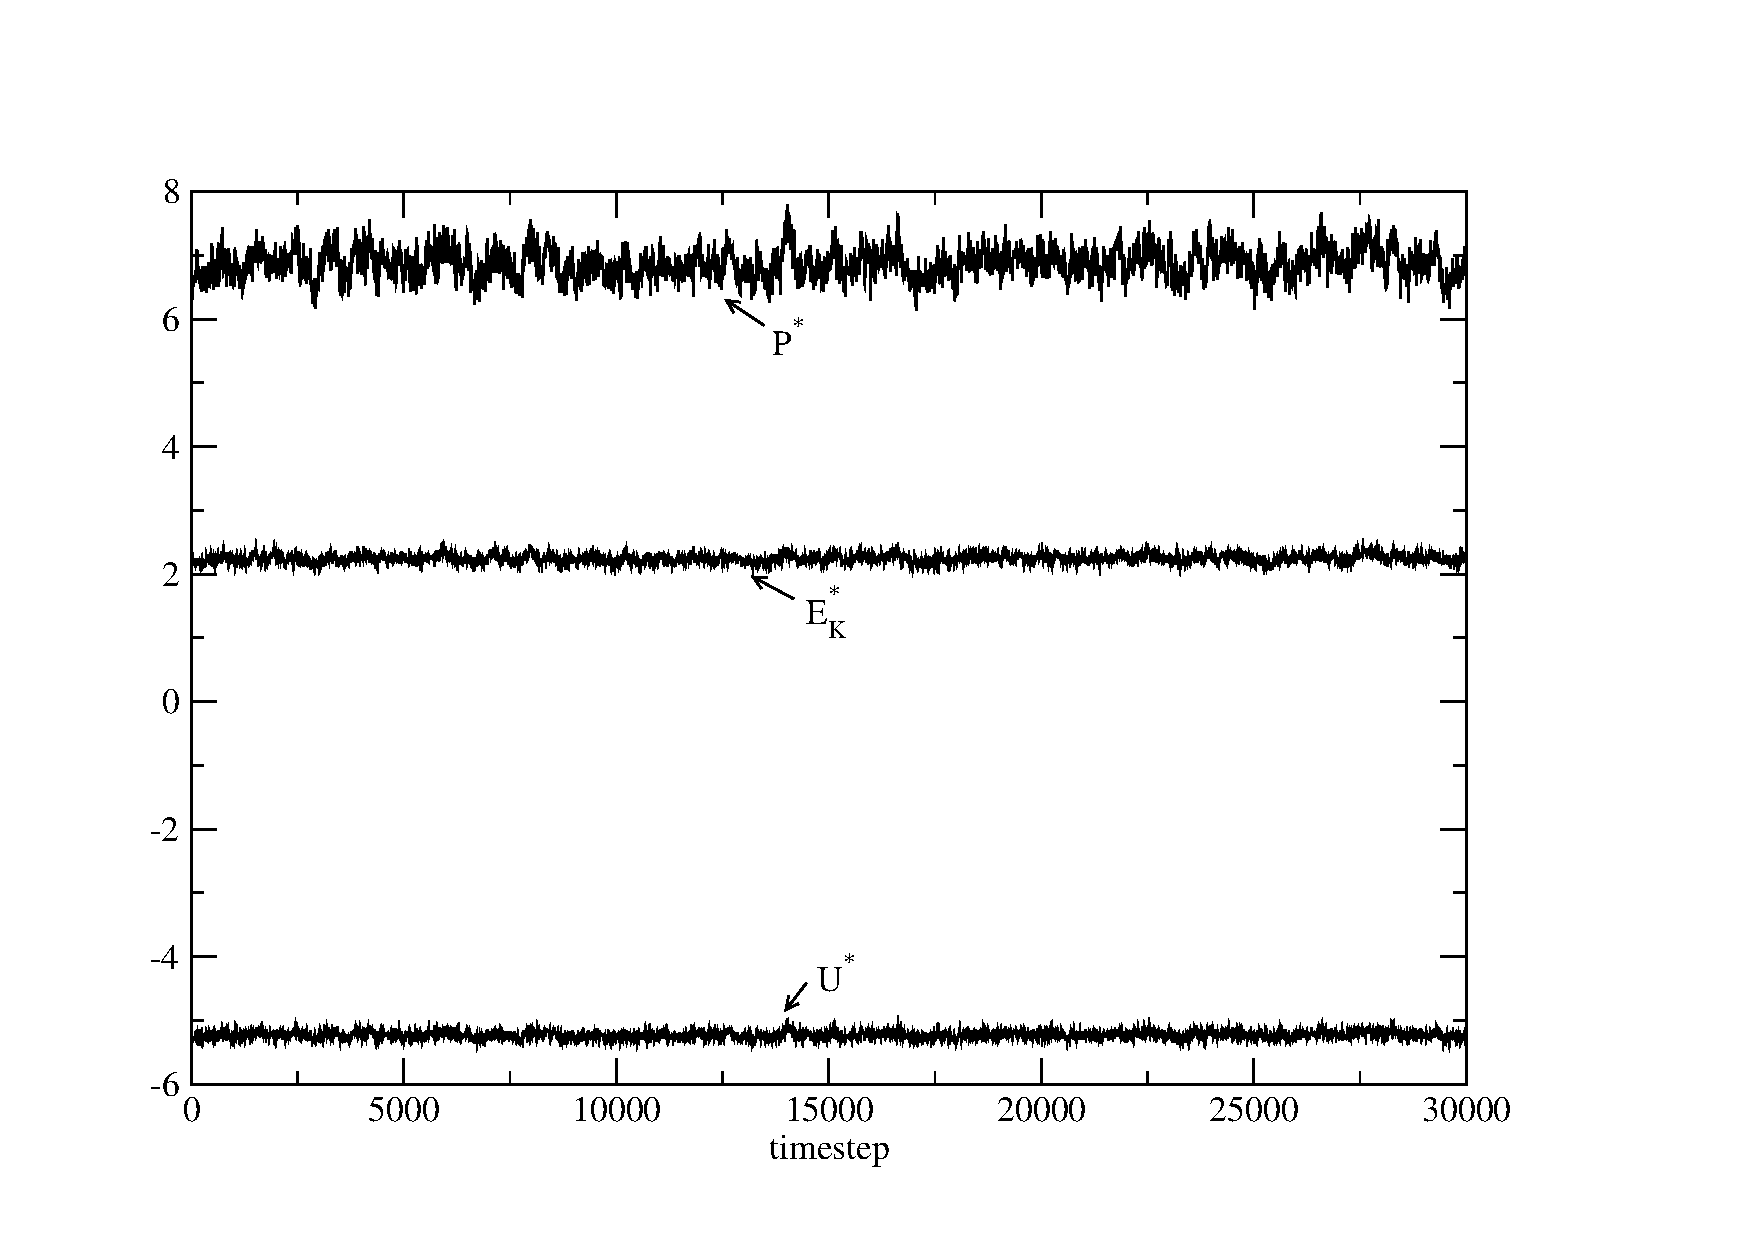
\includegraphics[clip,width=\textwidth]{figures/energyplot} 
    \caption{\label{fig:fluctuations} Plot showing flucuation of pressure
      ($P^*=P\sigma^3/\varepsilon$), kinetic energy per particle
      ($E_K^*=E_K/N\varepsilon$) and potential energy per particle
      ($U^*=U/N\varepsilon$).  Results are from a force-driven simulation
      involving 864 particles, at a density $\rho^*=0.9$ and
      temperature $\langle T\rangle=1.497$. Values were collected
      every 10 timesteps where each timestep was $\Delta t = 0.005$.}
  \end{center}
\end{figure}

\begin{equation}
  \label{eq:TAdef}
  \langle A \rangle = \lim_{t \to \infty} \frac{1}{t}  \int^{t_0+t}_{t_0}A(\tau) d\tau
\end{equation}

This time average can be calculated precisely in event-driven
simulations for several properties such as pressure, kinetic energy
and potential energy.  These only change at collisions and therefore
are constant for the time between the collision and can be calculated
by \eqref{eq:TASum}.

\begin{equation}
  \label{eq:TASum}
  \langle A \rangle = \frac{1}{t}\sum^{t_o+t}_{t_0}A(\tau)\Delta \tau
\end{equation}

In force-driven simulators all properties change continuously and
hence time averages cannot be calculated precisely, however
approximations can be made. If properties are measured every uniform
period of time, the time average can be approximated by equation
\eqref{eq:TAforcedriven}, where $M$ is the number of measurements
taken.

\begin{equation}
  \label{eq:TAforcedriven}
  \langle A \rangle = \frac{1}{M} \sum^{M}_{1}A(\tau)
\end{equation}
\section{Units}

In molecular dynamics simulations, properties are frequently measured
in dimensionless forms \cite{Haile1997}. These ``reduced units'' are
usually denoted with an asterisk.  In order to achieve this a number
of fundamental dimensions are needed: a characteristic length $\sigma$, a
characteristic energy $\varepsilon$, and the mass of one particle $m$.  In the case of
the Lennard-Jones potential, the characteristic length and energy are
taken as: the distance of the root, and the depth of the attractive
well respectively. A table of reduced forms are given in table
\ref{tab:reducedForms}.

\begin{table}[htp] 
  \caption{Table of reduced forms of various quanities used in this
    dissertation \cite{Haile1997}}
  \label{tab:reducedForms}
  \begin{center}
    \begin{tabular}{c c}
      \toprule
      Quantity & Reduced forms \\
      \midrule
      Density & $\rho^* = N \sigma^3 / V$ \\
      Energy & $E^* = E / \varepsilon$ \\
      Force & $F^* = F\sigma/\varepsilon$ \\
      Length & $r^* = r / \sigma$ \\
      Pressure & $P^* = P \sigma^3 /\varepsilon$ \\
      Temperature & $T^* = kT/\varepsilon$ \\
      Time & $t^* = t / (\sigma \sqrt{m/\varepsilon})$ \\
      Velocity & $v^* = v\sqrt{m/\varepsilon}$ \\
      \bottomrule
    \end{tabular}
  \end{center}
\end{table}

\section{Energy}
Perhaps one of the most important properties to measure in MD
simulations is the total internal energy of the system.  For isolated
systems, i.e.\ systems where mass or energy cannot enter or leave the
system, this internal energy is the sum of kinetic and potential
energy (equation \eqref{eq:internalE}).

\begin{equation}
  E = E_K + \mathcal{U} \label{eq:internalE}
\end{equation}

The total kinetic energy in the system is the sum of the kinetic
energy of each particle, as shown in equation \eqref{eq:totalEK}.

\begin{equation}
  \label{eq:totalEK}
  E_K = \sum_i^N mv_i^2
\end{equation}

The potential energy of the system is the sum of the potential energy
between every pair of particles (for a pairwise potential), and is
shown in equation \eqref{eq:totalU}.

\begin{equation}
  \label{eq:totalU}
  \mathcal{U} = \underset{i\;\;<\;\;j}{\sum\sum}\mathcal{U}(r_{ij})
\end{equation}

Event-driven simulators strictly conserve energy, therefore the
kinetic and potential energy can be measured at the beginning of the
simulation and then updated whenever either changes e.g.\ when a
collision occurs.

\section{Temperature}

The velocity distrubution of particles is given by the Maxwell
distribution \cite{Haile1997}, shown in equation
\eqref{eq:MaxwellDist}, where $k_B$ is the Boltzman Constant.

\begin{equation}
  \label{eq:MaxwellDist}
  f(v_x)dv_x = \sqrt{\frac{m}{2\pi k_BT}}e^{-\frac{mv_x^2}{2k_BT}} 
\end{equation}

This is the form of a Gaussian distribution and it can be shown
\cite{Landau1968} that the mean square velocity in any direction is as
shown in equation \eqref{eq:MSV}.

\begin{equation}
  \label{eq:MSV}
  \bar{\;v_x^2\;} = \frac{k_BT}{m}
\end{equation}

Making the assumption that the velocity distribution is the same in
each direction, the temperature can be expressed as equation
\eqref{eq:Temperature}, by taking the average temperature in each
direction. 

\begin{equation}
\label{eq:Temperature}
  T^* = k_BT = \frac{mv^2}{3N} = \frac{2}{3N}E_K
\end{equation}

This allows the calculation of the temperature from the kinetic energy
of the system.
\section{Pressure}

The pressure in a molecular dynamics simulation is calculated using
the virial equation of state (equation \eqref{eq:virialEOS}) \cite{Landau1968}.

\begin{equation}
  \label{eq:virialEOS}
  \frac{PV}{Nk_BT} = 1 + B_2\rho + B_3\rho^2 + B_4\rho^3 + ... + B_{n}\rho^{n-1}
\end{equation}

The coefficients, $B_2, B_3, B_4, ..., B_n$ are known as the second,
third, etc. virial coeffcients.  Values for these virial coefficients
are available in the literature for common potentials such as hard
spheres \cite{Labik2005} or Lennard-Jones
\cite{Schultz2009}. Physically these coefficients represent the
contribution to the pressure by two, three, etc particles interacting,
and since most potentials are pairwise the pressure contribution is
truncated at the second virial coefficient, the form of which in three
dimensions is given in equation \eqref{eq:secondVirial} \cite{Smith2005}.

\begin{equation}
  \label{eq:secondVirial}
  B_2 = -2\pi \int^\infty_0 \left(e^{\mathcal{U}(r)/kT}-1\right)r^2dr
\end{equation}

However these virial coefficients do not apply to molecular dynamics
simulations that use periodic boundary conditions \cite{Haile1997},
therefore an alternative method is required.

Using kinetic theory and measuring momentum flux during the simulation
an expression for the second virial coefficient can be created for
both simulation methods.  In force driven simulations, the second
virial can be calculated using equation \eqref{eq:virialMD}
\cite{Haile1997}.

\begin{equation}
  \label{eq:virialMD}
  B_2\rho = \frac{1}{3NkT}\left \langle\underset{i\;\;<\;\;j}{\sum\sum}\mathbf{F}_{ij}\cdot\mathbf{r}_{ij} \right\rangle
\end{equation}

Calculating the pressure in event-driven simulators is more complex
due to the lack of forces in the simulation, however by keeping track
of the momentum flux at each collision an average pressure can be
calculated using equation \eqref{eq:virialED}\cite{Lue2005}.  Here $N_{\text{coll}}$
is the total number of collisions during the time $t$.

\begin{equation}
  \label{eq:virialED}
  B_2\rho = \frac{m}{3}\frac{N_{\text{coll}}}{Nt}\langle\mathbf{r}_{ij}\cdot\Delta \mathbf{v}_i\rangle_{\text{coll}}
\end{equation}
\section{g(r)}
\section{g(r) to pressure and temperature}
\section{long range corrections}

\chapter{From Continuous to Discontinuous}
State the case why we want to run discontinuous systems, the
advantages (fast, extremely stable-> infinitely hard potentials, and
disadvantages (underdeveloped set of potentials in the literature,
complex algorithm). These disadvantages can be overcome by writing a
good general EDMD program and finding a a general method to convert
the hard work in soft potentials to stepped potentials. 


\chapter{Results} 

\section{Benchmarking} 

\subsection{Introduction} 
After a MD simulator has been created it is necessary to compare its
results with those generated by others, to verify that the simulator
works correctly.

\subsection{Force based code verusus NIST and ESpReSSo}

\subsection{Event Driven}
Event driven codes are significantly more complex than time-stepping codes, so we need more tests

{\bf HARD SPHERES v LEO}

{\bf Stepped Potential of Chapela}

\section{Chapela's dumb stepping and very good stepping versus force based. }

Show that dumb stepping doesn't work, show how good chapela's results actually are when he tries. Proves this is possible.

\section{Stepping in probability versus action}

Hard cores dominate the freezing behaviour (see Alder and Wainwrights
famous paper) and therefore for high density pressure etc. but the stepping in equal probability doesnt do this.

\section{Hard core position}

Try setting the inner step to infinite energy

Use barker henderson, an old attempt to make hard sphere match
everything else. (too far out).


talk about probability of finding a particle in the core. Talk about
sigma try out 3, 4, and 5.

\section{Temperature comparisons}
Show that chapelas solution gets worse faster than ours.

\subsection{Event-Driven Simulator}
 The event-driven simulator was first tested running a hard sphere
 simulation before testing the more complex stepped potentials. A
 single 'step' with a energy requirement sufficiently large such that
 no particle could enter it. The simulation was run once at a range of
 densities using 864 particles at a reduced temperature of $T^*=1$ for
 5 million collisions, the results were compared with those of Lue
 \cite{Lue2005} in table \ref{tab:benchhard}. The agreement between
 results is good and lies within statistical uncertainty. The largest
 discrepancies are in the values for the coefficient of diffusion at
 low densities which is probably due to Lue's values were obtained
 after 10 million collisions.

\begin{table} \caption{Comparison of results obtained by the event-driven
simulator with literature values. $t_{avg}$ is the average time
between collisions, $\langle\mathbf{\hat{r}} \cdot \Delta \mathbf{v}
\rangle_{coll}$ is the average momentum transfer per collision, and D
is the coefficient of
diffusion.} 
\label{tab:benchhard} 
\begin{center} 
  \begin{tabular}{l c c c c c c} 
    \toprule $\rho$ & \multicolumn{2}{c}{$t_{avg}$} &
      \multicolumn{2}{c}{$\langle\mathbf{\hat{r}} \cdot \Delta
        \mathbf{v} \rangle_{coll}$} & \multicolumn{2}{c}{D} \\ 
      \cmidrule(rl{0.75em}){2-3} 
      \cmidrule(rl{0.75em}){4-5}
      \cmidrule(rl{0.75em}){6-7} & Simulator & Lue & Simulator & Lue &
      Simulator & Lue
      \\ \midrule 0.3 & 0.3052 & 0.3052 & 1.775 & 1.772 & 0.53 & 0.55 
      \\ 0.4 & 0.1944 & 0.1942 & 1.776 & 1.773 & 0.341 & 0.359 
      \\ 0.5 & 0.13024 & 0.13031 & 1.774 & 1.7724 & 0.247 & 0.247 
      \\ 0.6 & 0.08966 & 0.08968 & 1.771 & 1.7721 & 0.169 & 0.173 
      \\ 0.7 & 0.0625 & 0.0625 & 1.773 & 1.776 & 0.114 & 0.113
      \\ 0.8 & 0.04365 & 0.0436 & 1.772 & 1.772 & 0.064 & 0.065 
      \\ 0.9 & 0.03029 & 0.03024 & 1.773 & 1.772 & 0.033 & 0.0327
      \\ \bottomrule
    \end{tabular} 
  \end{center} 
\end{table}

The simulator was then benchmarked using a step potential. The results
were compared with Chapela et al \cite{Chapela1989} using their 'Case
6' steps. The simulation was run for 1.5 million collisions using 864
particles. Each simulation was run ten times and the mean values and
standard deviations are given in table
\ref{tab:benchsoft} 

\begin{table} 
  \caption{Comparison of results
    obtained by the event-driven simulator with literature values
    using stepped potentials. Numbers in parenthesis indicate the
    uncertainty in the final digit.
\label{tab:benchsoft}} 
  \begin{center} 
    \begin{tabular}{l c c c c c c} 
      \toprule
      $\rho$ & \multicolumn{2}{c}{$\langle T\rangle$} &
      \multicolumn{2}{c}{$\langle U \rangle$} &
      \multicolumn{2}{c}{$\langle P \rangle$}
      \\ \cmidrule(rl{0.75em}){2-3} \cmidrule(rl{0.75em}){4-5}
      \cmidrule(rl{0.75em}){6-7}& Simulator & Chapela et al &
      Simulator & Chapela et al & Simulator & Chapela etal\\ 
      \midrule
      0.85 & 0.719(3) & 0.72 & -6.04(7) & -5.80 & -0.5(4) & 0.54
      \\ 0.85& 1.339(8) & 1.34 & -5.130(9) & -5.14 & 4.08(4) & 4.08
      \\ 0.85 & 2.35(1) & 2.35 & -4.24(2) & -4.20 & 8.78(9) & 8.86
      \\ 0.85 & 3.37(2) & 3.37 & -3.48(2) & -3.49 & 12.90(9) & 13.00
      \\ 0.85 & 4.59(1) & 4.60 & -2.67(1) & -2.68 & 17.31(8) & 13.43
      \\ 0.75 & 0.811(2) & 0.81 & -5.095(3) & -5.08 & -0.20(2) & -0.24
      \\ 0.75 &1.309(9) & 1.31 & -4.67(1) & -4.63 & 1.81(5) & 1.84
      \\ 0.75 & 2.49(1) & 2.49 & -3.88(1) & -3.82 & 5.80(4) & 5.95
      \\ 0.75 & 3.59(2) & 3.59 & -3.26(1) & -3.22 & 9.03(7) & 9.20
      \\ 0.65 & 1.309(8) & 1.31 & -4.081(8) & -4.06 & 0.80(3) & 0.81
      \\0.65 & 2.61(1) & 2.61 & -3.42(1) & -3.41 & 3.86(5) & 3.89
      \\ 0.65 & 3.79(1) & 3.79 & -2.926(9) & -2.94 & 6.34(7) & 6.33
      \\ 
      \bottomrule 
    \end{tabular}
\end{center} 
\end{table} 

%\section{Adding Figures} 
%To add figures to yourtext,you need to use a series of commands, but 
%you can just copy paste the one below and tweak it for your needs. 
%\begin{figure}[htp] 
% \centering 
%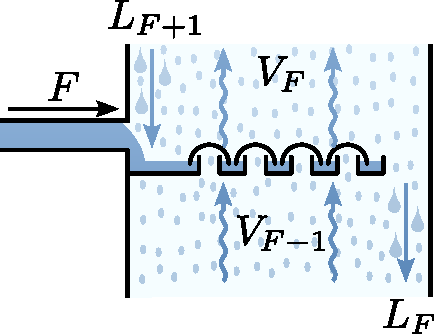
\includegraphics[clip,width=0.5\textwidth]{figures/testfig} 
%\caption{\label{fig:testfig} A test figure.} 
%\end{figure}


% %\section{References} 
%You can reference entries in your bib file using the key you have set 
%for it like so~\cite{Bannerman_2009}. I can even do cool things like 
%say the author of that citation is \citeauthor{Bannerman_2009} and it 
%was published in \citeyear{Bannerman_2009}. Or even ask for a full
%citation, like so: \fullcite{Bannerman_2009}. % 
%But you must remember toprintthe bibliography at the end of every 
%chapter!
\newpage\printbibliography[heading=thesisChapterBib] 

\appendix
\chapter{Derivation of Collision Dynamics for Stepped Potentials}
Considering a collision between particles $i$ and $j$, each with mass,
$m$ with a step energy difference of $\Delta U$, the conservation of
momentum is shown in equation \eqref{eq:consMom}. Here the prime
indicates post-collision values.

\begin{equation}
\label{eq:consMom}
m\mathbf{v}_i + m\mathbf{v}_j = m\mathbf{v}'_i + m\mathbf{v}'_j
\end{equation}

The momentum change of each particle must occur along the separation
vector between the two particles, which can be expressed by equation
\eqref{eq:defA}, where $A$ is an arbitary coefficient.

\begin{equation}
  \label{eq:defA}
  m\mathbf{v}_i - m\mathbf{v}'_i = -(m\mathbf{v}_j - m\mathbf{v}'_j) 
  = -A\mathbf{\hat{r}}_{ij}
\end{equation}

Energy must also be conserved in the system so equation
\eqref{eq:constE} must also apply.  This can be rewritten to equations
\eqref{eq:constE1} and \eqref{eq:constE2}

\begin{equation}
  \label{eq:constE}
  \frac{1}{2}mv_i^2 + \frac{1}{2}mv_j^2 =
  \frac{1}{2}m{v'_i}^2 + \frac{1}{2}m{v'_j}^2 + \Delta U
\end{equation}

\begin{equation}
  \label{eq:constE1}
  v_i^2 - {v'_i}^2 +
  v_j^2 - {v'_j}^2 - \frac{2}{m}\Delta U = 0
\end{equation}

\begin{equation}
  \label{eq:constE2}
  (\mathbf{v}_i - \mathbf{v}'_i)\cdot(\mathbf{v}_i + \mathbf{v}'_i) +
  (\mathbf{v}_j - \mathbf{v}'_j)\cdot(\mathbf{v}_j + \mathbf{v}'_j) -
  \frac{2}{m}\Delta U = 0
\end{equation}

Equation \eqref{eq:defA} can now be substituted into
\eqref{eq:constE2} to give equation \eqref{eq:eq1}.

\begin{equation}
  \label{eq:eq1}
  \frac{A}{m}\mathbf{\hat{r}}_{ij} (\mathbf{v}_j - \mathbf{v}_i 
  + \mathbf{v}'_j - \mathbf{v}'_i) - \frac{2}{m}\Delta U = 0
\end{equation}

Equation \eqref{eq:defA} and the definition of the separation velocity
vector ($\mathbf{v}_{ij} = \mathbf{v}_i - \mathbf{v}_j$) can be
substituted into equation \eqref{eq:eq1} to give \eqref{eq:eq2}.

\begin{equation}
  \label{eq:eq2}
  -\frac{A^2}{m}
  -A\mathbf{\hat{r}}_{ij}\cdot\mathbf{v}_{ij} - \Delta U = 0
\end{equation}

This is a quadratic equation in terms of $A$ therefore it's roots must
be given by equation \eqref{eq:devQuadratic}.

\begin{equation}
  \label{eq:devQuadratic}
  A = -\frac{m}{2}\left((\mathbf{v}_{ij}\cdot\mathbf{\hat{r}}_{ij}) \pm
  \sqrt{(\mathbf{v}_{ij}\cdot\mathbf{\hat{r}}_{ij})^2 - \frac{4}{m}\Delta U}\right)
\end{equation}  

From equation \eqref{eq:defA}, the change in velocity of each particle
is given in equations \eqref{eq:deltaV}

\begin{subequations}
  \label{eq:deltaV}
  \begin{align}
    \Delta\mathbf{v}_i &= \frac{A}{m} \mathbf{\hat{r}}_{ij} \\
    \Delta\mathbf{v}_j &= -\frac{A}{m}\mathbf{\hat{r}}_{ij}    
  \end{align}
\end{subequations}

\end{document}

%%%%TAYLOR SERIES FOR GEAR'S ALGORITHM%%%% %\begin{equation} 
%\begin{aligned}
%\vec{r}(t+\Delta t) &= \vec{r}(t) + \vec{v}(t) \Delta t 
% +\frac{1}{2}\vec{a}(t)\Delta t^2 + \frac{1}{3!}\vec{b}(t)\Delta t^3 
% +\frac{1}{4!}\vec{c}(t)\Delta t^4 + \frac{1}{5!}\vec{d}(t)\Delta t^5 \\
%\vec{v}(t+\Delta t) &= \vec{v}(t) \Delta t + \vec{a}(t)\Delta t^2 
% +\frac{1}{2}\vec{b}(t)\Delta t^3 + \frac{1}{3!}\vec{c}(t)\Delta t^4 +
%\frac{1}{4!}\vec{d}(t)\Delta t^5 \\ %\vec{a}(t+\Delta t) &= \vec{a}(t)\Delta
%t^2+ \vec{b}(t)\Delta t^3 % + \frac{1}{2!}\vec{c}(t)\Delta t^4 +
%\frac{1}{3!}\vec{d}(t)\Delta t^5 \\ %\vec{b}(t+\Delta t) &= \vec{b}(t)\Delta
%t^3+ \vec{c}(t)\Delta t^4 % + \frac{1}{2!}\vec{d}(t)\Delta t^5 \\
%\vec{c}(t+\Deltat) &= \vec{c}(t)\Delta t^4 + \vec{d}(t)\Delta t^5 \\
%\vec{d}(t+\Delta t) &=
%\vec{d}(t)\Delta t^5 \\ %\end{aligned} %\end{equation}
